% ----------------------------------------------------------------- %
%             The Speech Signal Processing Toolkit (SPTK)           %
%             developed by SPTK Working Group                       %
%             http://sp-tk.sourceforge.net/                         %
% ----------------------------------------------------------------- %
%                                                                   %
%  Copyright (c) 1984-2007  Tokyo Institute of Technology           %
%                           Interdisciplinary Graduate School of    %
%                           Science and Engineering                 %
%                                                                   %
%                1996-2016  Nagoya Institute of Technology          %
%                           Department of Computer Science          %
%                                                                   %
% All rights reserved.                                              %
%                                                                   %
% Redistribution and use in source and binary forms, with or        %
% without modification, are permitted provided that the following   %
% conditions are met:                                               %
%                                                                   %
% - Redistributions of source code must retain the above copyright  %
%   notice, this list of conditions and the following disclaimer.   %
% - Redistributions in binary form must reproduce the above         %
%   copyright notice, this list of conditions and the following     %
%   disclaimer in the documentation and/or other materials provided %
%   with the distribution.                                          %
% - Neither the name of the SPTK working group nor the names of its %
%   contributors may be used to endorse or promote products derived %
%   from this software without specific prior written permission.   %
%                                                                   %
% THIS SOFTWARE IS PROVIDED BY THE COPYRIGHT HOLDERS AND            %
% CONTRIBUTORS "AS IS" AND ANY EXPRESS OR IMPLIED WARRANTIES,       %
% INCLUDING, BUT NOT LIMITED TO, THE IMPLIED WARRANTIES OF          %
% MERCHANTABILITY AND FITNESS FOR A PARTICULAR PURPOSE ARE          %
% DISCLAIMED. IN NO EVENT SHALL THE COPYRIGHT OWNER OR CONTRIBUTORS %
% BE LIABLE FOR ANY DIRECT, INDIRECT, INCIDENTAL, SPECIAL,          %
% EXEMPLARY, OR CONSEQUENTIAL DAMAGES (INCLUDING, BUT NOT LIMITED   %
% TO, PROCUREMENT OF SUBSTITUTE GOODS OR SERVICES; LOSS OF USE,     %
% DATA, OR PROFITS; OR BUSINESS INTERRUPTION) HOWEVER CAUSED AND ON %
% ANY THEORY OF LIABILITY, WHETHER IN CONTRACT, STRICT LIABILITY,   %
% OR TORT (INCLUDING NEGLIGENCE OR OTHERWISE) ARISING IN ANY WAY    %
% OUT OF THE USE OF THIS SOFTWARE, EVEN IF ADVISED OF THE           %
% POSSIBILITY OF SUCH DAMAGE.                                       %
% ----------------------------------------------------------------- %
\hypertarget{vopr}{}
\name{vopr}{execute vector operations}{number operation}

\begin{synopsis}
\item[vopr] [ --l $L$ ] [ --n $N$ ] [ --i ] [ --a ] [ --s ] [ --m ] [ --d ]
 [ --ATAN2 ] [ --AM ] [ --GM ]
 \item[\ ~~~~] [ --gt ] [--ge ] [ --lt ] [--le] [ --eq ] [ --ne ]
 [ {\em file1} ] [ {\em infile} ]
\end{synopsis}

\begin{qsection}{DESCRIPTION}
This command performs vector operations in input files.
In other words
\begin{description}
\itemb{\em file1}
first vector file (if it is not assigned then stdin)
\itemb{\em infile}
second vector file (if it is not assigned then stdin)
\end{description}
the first file gives the operation vectors {\bf a}
and the second file gives the operation vectors {\bf b}.
The assigned operation is undertaken and the results
are sent to the standard output.
\par
Input and output data are in float format.
\par
The undertaken action depends on the number of assigned files
as well as the vector lengths as exemplified in the following.
\par
If two files are assigned (when only one file is assigned,
it is assumed that it corresponds to {\em infile}) then,
depending on the vector sizes, the following actions
are taken.
\begin{description}
\item{when $L=1$}~\\
\begin{tabular}{l|c|c|c|c|c} \cline{2-6}
{\em file1} (stdin)     & {$a_1$} & {$a_2$} & {\dots}
                        & {$a_i$} & {\dots} \\ \cline{2-6}
\multicolumn{6}{c}{}    \\[-10pt] \cline{2-6}
{\em infile}            & {$b_1$} & {$b_2$} & {\dots}
                        & {$b_i$} & {\dots} \\ \cline{2-6}
\multicolumn{6}{c}{}    \\[-10pt] \cline{2-6}
{\em Output} (stdout)   & {$y_1$} & {$y_2$} & {\dots}
                        & {$y_i$} & {\dots} \\ \cline{2-6}
\end{tabular}
\par
One data from one file corresponds to one data on the other file.
\item{when $L\geq 2$}~\\
\begin{tabular}{l|c|c|c|l} \cline{2-5}
{\em file1} (stdin)     & {$a_{11}$,\dots,$a_{1L}$}
                        & {$a_{21}$,\dots,$a_{2L}$}
                        & {$a_{31}$,\dots,$a_{3L}$}
                        & {$a_{41}$,\dots} \\ \cline{2-5}
\multicolumn{5}{c}{}    \\[-10pt]
                        \cline{2-2}
{\em infile}            & {$b_{1}$,\dots,$b_{L}$}
                        & \multicolumn{3}{c}{} \\ \cline{2-2}
\multicolumn{5}{c}{}    \\[-10pt]
                        \cline{2-5}                     
{\em Output} (stdout)   & {$y_{11}$,\dots,$y_{1L}$}
                        & {$y_{21}$,\dots,$y_{2L}$}
                        & {$y_{31}$,\dots,$y_{3L}$}
                        & {$y_{41}$,\dots} \\ \cline{2-5}
\end{tabular}
\par
In this case, the operation vector is read only once from
{\em infile}, and the operations are recursively performed.
\end{description}
\par
When the information related to {\bf a} and {\bf b} is contained
in a single file,
(if only one file is assigned,
or if no file assignment is made),
the --i option should be used
and the action does not depend on the vector length.
\begin{description}
\item{when $L\geq 1$}~\\
\begin{tabular}{l|c|c|c|c|l} \cline{2-6}
{\em file} (stdin)      & {$a_{11}$,\dots,$a_{1L}$}
                        & {$b_{11}$,\dots,$b_{1L}$}
                        & {$a_{21}$,\dots,$a_{2L}$}
                        & {$b_{21}$,\dots,$b_{2L}$}
                        & ~~~ \\ \cline{2-6}
%                       & {$a_{31}$,\dots} \\ \cline{2-6}
\multicolumn{6}{c}{}    \\[-10pt]
                        \cline{2-2} \cline{4-4} \cline{6-6}
{\em Output} (stdout)   & {$y_{11}$,\dots,$y_{1L}$} &
                        & {$y_{21}$,\dots,$y_{2L}$} &
                        & ~~~ \\
%                       & {$y_{31}$,\dots} \\
                        \cline{2-2} \cline{4-4} \cline{6-6}
\end{tabular}
\par
Input vectors are read from a single file.
\end{description}
\end{qsection}

\begin{options}
 \argm{l}{L}{length of vector}{1}
 \argm{n}{N}{order of vector}{L-1}
 \argm{i}{}{when a single file file is specified,
 the file contains a and b.}{FALSE}
 \argm{a}{}{addition $y_i=a_i+b_i$}{FALSE}
 \argm{s}{}{subtraction $y_i=a_i-b_i$}{FALSE}
 \argm{m}{}{multiplication $y_i=a_i*b_i$}{FALSE}
 \argm{d}{}{division $y_i=a_i/b_i$}{FALSE}
 \argm{ATAN2}{}{atan2 $y_i=\atan2(b_i,a_i)$}{FALSE}
 \argm{AM}{}{arithmetic mean $y_i=(a_i + b_i) / 2$}{FALSE}
 \argm{GM}{}{geometric  mean $y_i=\sqrt{a_i * b_i}$}{FALSE}
 \argm{c}{}{choose smaller value}{FALSE}
 \argm{f}{}{choose larger value}{FALSE}
 \argm{gt}{}{decide ``greater than''}{FALSE}
 \argm{ge}{}{decide ``greater than or equal''}{FALSE}
 \argm{lt}{}{decide ``less than''}{FALSE}
 \argm{le}{}{decide ``less than or equal''}{FALSE}
 \argm{eq}{}{decide ``equal to''}{FALSE}
 \argm{ne}{}{decide ``not equal to''}{FALSE}
\end{options}

\begin{qsection}{EXAMPLE}
The output file {\em data.c} contains addition of
vectors in float format read from {\em data.a} and {\em data.b}:
\begin{quote}
  \verb!vopr -a data.a data.b > data.c !
\end{quote}
\par
In the following example, a sin wave is passed through
a window with length 256 and coefficients given from
{\em data.w}:
\begin{quote}
  \verb!sin -p 30 -l 1000 | vopr data.w -l 256 -m | fdrw | xgr!
\end{quote}
\begin{center}
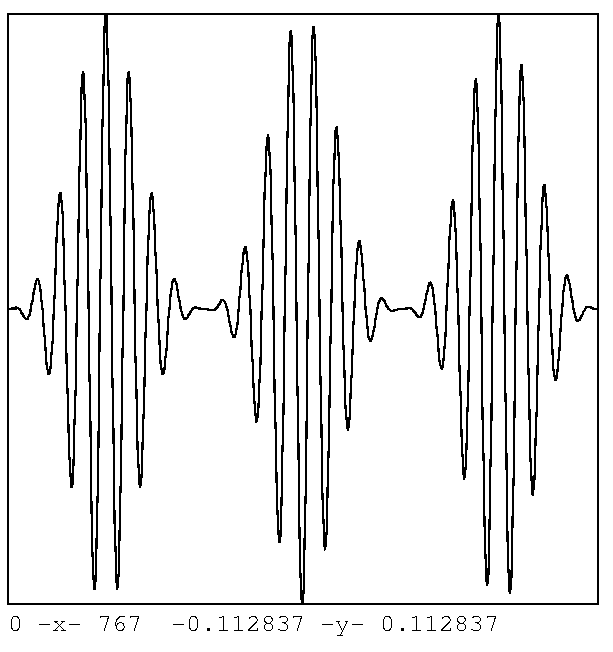
\includegraphics[width=6cm]{fig/vopr_1.pdf}
\end{center}
Similar results as from the above example can be obtained using the following:
 Here, it is considered that the contents of {\em data.w} correspond to a Blackman window:
\begin{quote}
  \verb!sin -p 30 -l 1000 | window | fdrw | xgr!
\end{quote}
\begin{center}
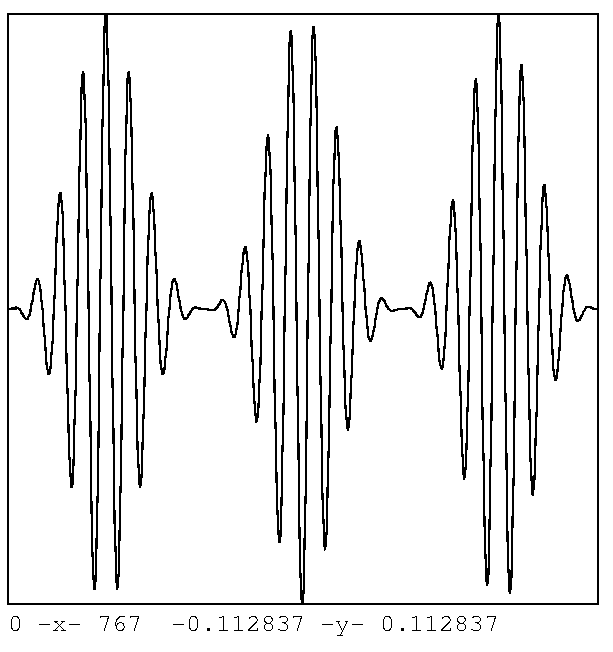
\includegraphics[width=6cm]{fig/vopr_2.pdf}
\end{center}
For other examples, suppose {\em data.a} contains
\begin{displaymath}
  1, 2, 3, 4, 5, 6, 7
\end{displaymath}
in float format and {\em data.b} contains
\begin{displaymath}
  3, 2, 1, 0, 5, 6, 7
\end{displaymath}
in float format.
In the following example,
smaller scalar values can be taken from
{\em data.a} and {\em data.b}, and
the result is sent to {\em data.c} in float format.
\begin{quote}
  \verb!vopr -c data.b < data.a > data.c !
\end{quote}
The output file {\em data.c} contains
\begin{displaymath}
  1, 2, 1, 0, 5, 6, 7.
\end{displaymath}
When executing following command line,
\begin{quote}
  \verb!vopr -ge data.b < data.a > data.c !
\end{quote}
the output file {\em data.c} contains:
\begin{displaymath}
  0.0, 1.0, 1.0, 1.0, 1.0, 1.0, 1.0
\end{displaymath}
On the other hand, when executing following command line,
\begin{quote}
  \verb!vopr -gt data.b < data.a > data.c !
\end{quote}
the output file {\em data.c} contains:
\begin{displaymath}
  0.0, 0.0, 1.0, 1.0, 0.0, 0.0, 0.0
\end{displaymath}
Moreover, when executing following command line,
\begin{quote}
  \verb!vopr -eq data.b < data.a > data.c !
\end{quote}
the output file {\em data.c} contains:
\begin{displaymath}
  0.0, 1.0, 0.0, 0.0, 1.0, 1.0, 1.0
\end{displaymath}
\end{qsection}

\begin{qsection}{NOTICE}
When both --l and --n are specified, latter argument is adopted.
\end{qsection}

\begin{qsection}{SEE ALSO}
\hyperlink{sopr}{sopr},
\hyperlink{vsum}{vsum}
\end{qsection}
